\documentclass{cmc}
\usepackage{makecell}
\begin{document}

\pagestyle{fancy}
\lhead{\textit{\textbf{Computational Motor Control, Spring 2022} \\
    Final project, Project 1, GRADED}} \rhead{Student \\ Names}

\section*{Student names: \ldots (please update)}

\textit{Instructions: Update this file (or recreate a similar one, e.g.\ in
  Word) to prepare your answers to the questions. Feel free to add text,
  equations and figures as needed. Hand-written notes, e.g.\ for the development
  of equations, can also be included e.g.\ as pictures (from your cell phone or
  from a scanner).  \textbf{\corr{This lab is graded.}} and needs to be
  submitted before the \textbf{\corr{Deadline : Wednesday 18-05-2022 23:59. You
      only need to submit one final report for all of the following exercises
      combined henceforth.}} Please submit both the source file (*.doc/*.tex)
  and a pdf of your document, as well as all the used and updated Python
  functions in a single zipped file called
  \corr{final\_report\_name1\_name2\_name3.zip} where name\# are the team
  member’s last names.  \corr{Please submit only one report per team!}}
\\

\section*{Swimming with Salamandra robotica – CPG Model}
\label{sec:exploring-swimming}

In this project you will control a salamander-like robot Salamandra robotica II
for which you will use Python and the MuJoCo physics engine. Now you have an
opportunity to use what you’ve learned to make the robot swim and eventually
walk. In order to do this, you should implement a CPG based controller,
similarly to the architecture shown in Figure~\ref{fig:controller-model}. Note
that the robot model used in this project has 8 joints along the body instead of
the 10 shown in Figure~\ref{fig:controller-model} thus the controller should be
implemented accordingly.

The project is based on the research of \cite{Crespi2013},
\cite{Karakasiliotis2013}, \cite{ijspeert2007swimming} and
\cite{thandiackal2021emergence}. It is strongly recommended to review
\cite{ijspeert2007swimming} and its supplementary material provided on
Moodle. You will be tasked with replicating and studying the Central Pattern
Generator (CPG).

\corr{\textit{NOTE:}} The session this week will be an introduction to the first
project. You will start by getting familiar with the code and implementing the
CPG network and eventually control the robot. While the MuJoCo simulator will
not be necessary yet, we recommend verifying you can install and run it before
the next session. Please get in contacts with the TAs if you need any
assistance. We also recommend that you implement the controller by Thursday
28-04-2022 such that you can proceed to the simulation experiment during the
next session.

\begin{figure}[h]
  \centering
  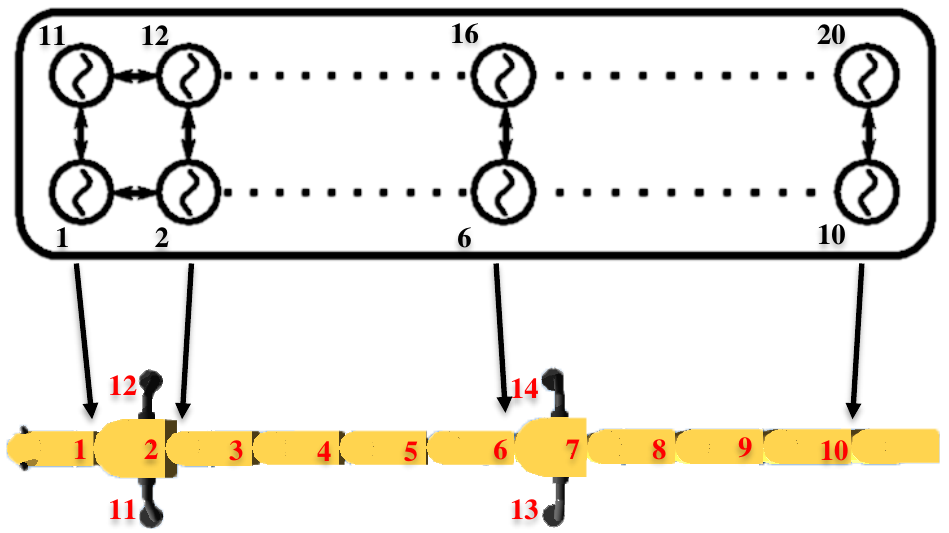
\includegraphics[width=0.5\textwidth]{figures/model_controller.png}
  \caption[Controller model]{A double chain of oscillators controlling
    the robot’s spine.}
  \label{fig:controller-model}
\end{figure}

\begin{figure}[ht]
  \centering 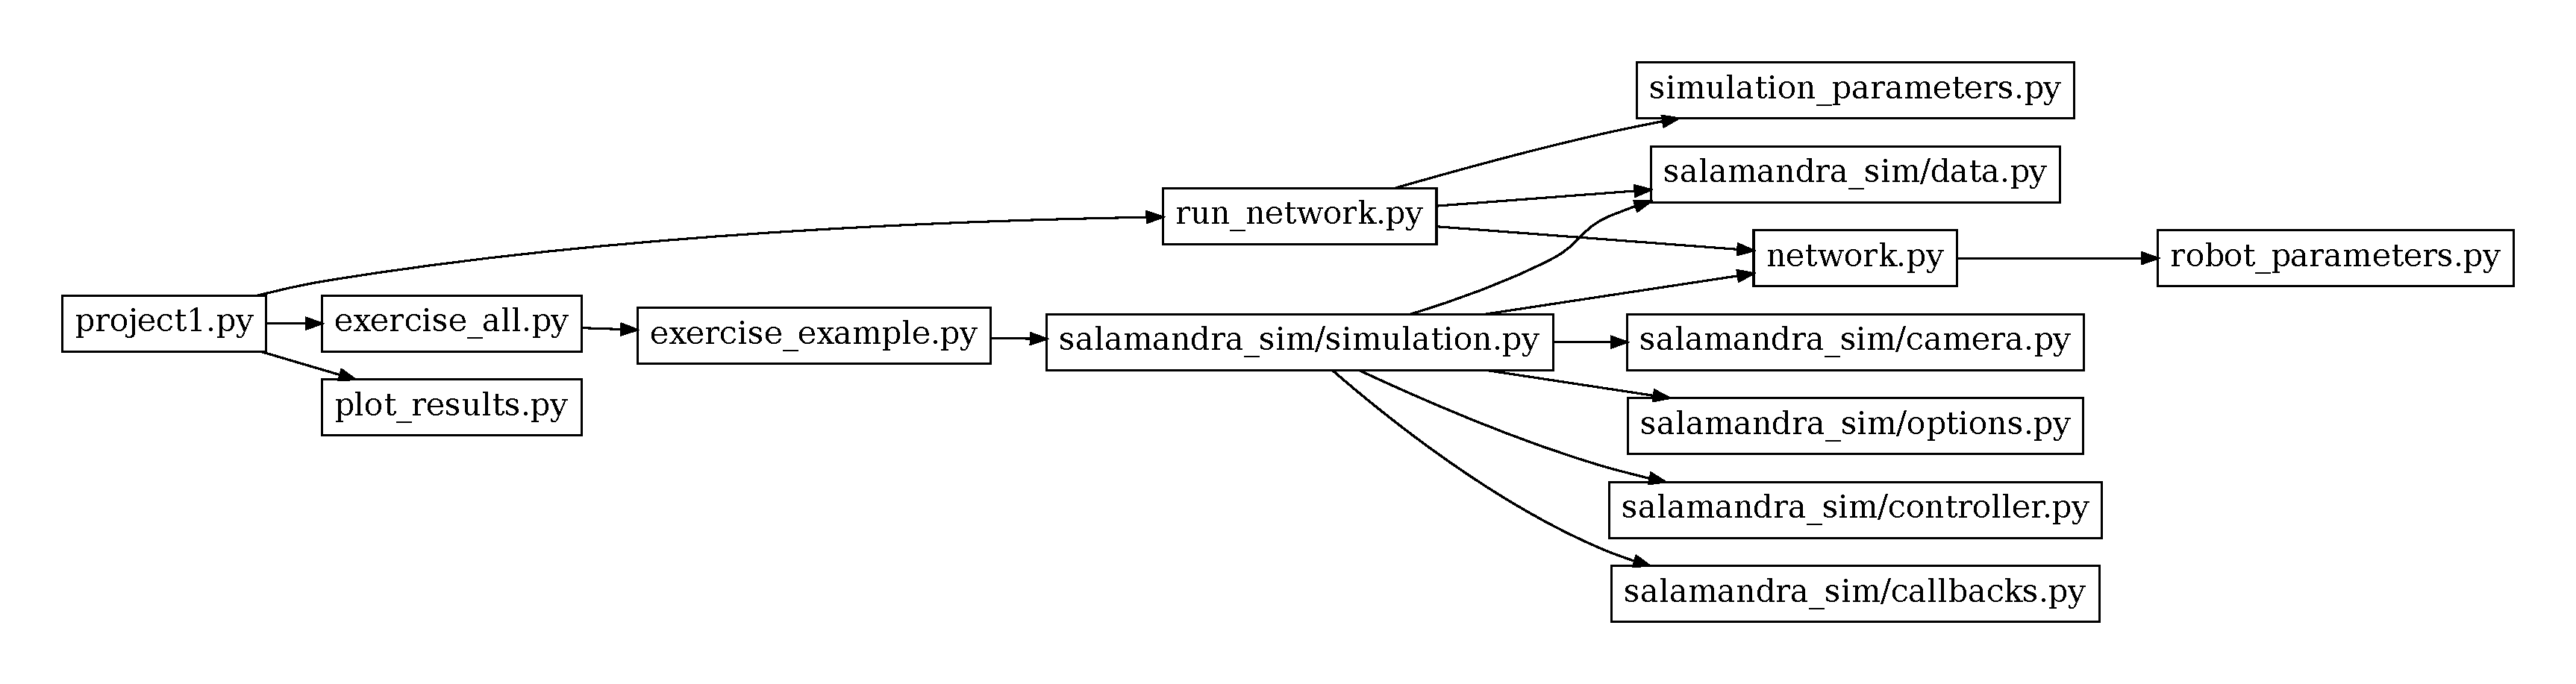
\includegraphics[width=1.0\textwidth]{figures/files}
  \caption{\label{fig:files} Exercise files dependencies. In this lab, you will
    be modifying \fileref{run\_network.py}, \fileref{network.py},
    \fileref{robot\_parameters.py} and \fileref{simulation\_parameters.py}}
\end{figure}

% \newpage

\subsection*{Code organization}
\label{subsec:code}

\begin{itemize}
\item \corr{\textbf{project1.py}} - A convenient file for running the entire
  project. Note you can also run the different exercises in parallel by
  activating \texttt{parallel=True}. \textit{You do not need to modify this
    file.}
\item \corr{\textbf{exercise\_all.py}} - Another convenient file for running all
  or specified exercises depending on arguments provided. \textit{You do not
    need to modify this file.}
\item \corr{\textbf{network.py}} - This file contains the different classes and
  functions for the CPG network and the Ordinary Differential Equations
  (ODEs). You can implement the network parameters and the ODEs here. Note that
  some parameters can be obtained from robot\_parameters.py to help you control
  the values.
\item \corr{\textbf{robot\_parameters.py}} - This file contains the different
  classes and functions for the parameters of the robot, including the CPG
  network parameters. You can implement the network parameters here. Note that
  some parameters can be obtained from the SimulationParameters class in
  \corr{simulation\_parameters.py} and provided in \corr{exercise\_\#.py} to
  help you control the values (refer to example.py).
\item \corr{\textbf{simulation\_parameters.py}} - This file contains the
  SimulationParameters class and is provided for convenience to send parameters
  to the setup of the network in \corr{network.py::SalamandraNetwork} via the
  robot parameters in \corr{robot\_parameters.py::RobotParameters}. The
  SimulationParameters is also intended to be used for experiment-specific
  parameters for the exercises. All the values provided in SimulationParameters
  are logged for each simulation, so you can also reload these parameters when
  analyzing the results of an experiment.
\item \corr{\textbf{run\_network.py}} - By running the script from Python,
  MuJoCo will be bypassed and you will run the network without a physics
  simulation. Make sure to use this file for question 8a to help you with
  setting up the CPG network equations and parameters and to analyze its
  behavior. This is useful for debugging purposes and rapid controller
  development since running the MuJoCo simulation takes more time.
\item \corr{\textbf{exercise\_example.py}} - Contains the example code structure
  to help you familiarize with the other exercises. \textit{You do not need to
    modify this file.}
\item \corr{\textbf{exercise\_\#.py}} - To be used to implement and answer the
  respective exercise questions. Note that \corr{exercise\_example.py} is
  provided as an example to show how to run a parameter sweep. Note that network
  parameters can be provided here.
\item \corr{\textbf{exercise\_all.py}} - A convenient file for running different
  exercises depending on arguments. See \corr{\textbf{lab8.py}} for an example
  on how to call it. \textit{You do not need to modify this file.}
\item \corr{\textbf{plot\_results.py}} - Use this file to load and plot the
  results from the simulation. This code runs with the original example provided
  and provides examples on how to collect the data.
\item \corr{\textbf{salamandra\_simulation folder}} - Contains all the remaining
  scripts for setting up and running the simulation experiments. \textit{You do
    not need to modify any of these file but should still go through them to get
    a better understanding of the code.}
\end{itemize}

% \newpage


\subsection*{Running the simulation}
You can run a simulation example with \corr{\textbf{exercise\_example.py}}. You
should see the Salamandra robotica model floating on the water. At this point
you can now start to work on implementing your exercises. Note that it is still
possible to proceed with exercise 8a if the simulator is not installed yet.

% \newpage

\section*{Questions}

The exercises are organized such that you will have to first implement the
oscillator network model in \corr{run\_network.py} code and analyze it before
connecting it to the body in the physics simulation.  Exercise 8a describes the
questions needed to implement the oscillator models. After completing exercise
8a you should have an oscillator network including both the spinal CPG and limb
CPG. Using the network implemented in exercise 8a you can explore the swimming,
walking and transition behaviors in the Salamandra robotica II model using the
MuJoCo simulation and complete the exercises that will be distributed next time.

\subsection*{8a. Implement a double chain of oscillators along with
  limb CPG's}
\label{sec:implement-chain}

Salamandra robotica has 8 joints along its spine and 1 joint for each
limb. The controller is defined as

\begin{equation}
  \label{eq:dphase}
  \dot{\theta}_i = 2 \pi f + \sum_j r_j w_{ij} sin(\theta_j - \theta_i - \phi_{ij})
\end{equation}

\begin{equation}
  \label{eq:dr}
  \dot{r}_i = a (R_i - r_i)
\end{equation}

\begin{equation}
  \label{eq:output}
  q_i = r_i(1 + cos(\theta_i)) - r_{i+8}(1 + cos(\theta_{i+8})) \text{ if body joint}
\end{equation}

with $ \theta_i $ the oscillator phase, f the frequency, $ w_{ij} $ the coupling
weights, $ \phi_{ij} $ the nominal phase lag (phase bias), $ r_i $ the
oscillator amplitude, $ R_i $ the nominal amplitude, $ a $ the convergence
factor and $ q_i $ the spinal joint angles. For more information, please refer
to \cite{ijspeert2007swimming}. Also note how these are the same equations,
although Equation \eqref{eq:dr} has been simplified into a first order ODE in
order to simplify the implementation in this project.


\begin{enumerate}
\item Implement the double chain oscillator model using the functions
  \fileref{network.py::network\_ode}. Test your implementation by running the
  network using \fileref{run\_network.py}. For the network parameters check
  lecture slides (pay attention to different number of segments). You can also
  find more information in \cite{ijspeert2007swimming} (especially in the
  supplementary material). You can set all the network parameters in the
  \fileref{robot\_parameters.py::RobotParameters}. To facilitate your work, you
  could start by only implementing the network for the body oscillators
  ($i=[0, ..., 15]$) and ignoring the leg oscillators ($i=[16, ..., 20]$). Refer
  to \corr{salamandra\_simulation/data.py::SalamandraState} and
  \corr{robot\_parameters.py::}\-\corr{RobotParameters} for the dimensions of
  the state and the network parameters respectively.

\item Implement the output of your CPG network to generate the spinal joint
  angles according to equation \ref{eq:output}. Implement this in the function
  \fileref{network.py::motor\_output}. Verify your implementation in by running
  the Python file \fileref{run\_network.py}.


\item Implement a drive and show that your network can generate swimming and
  walking patterns similarly to \cite{ijspeert2007swimming}. Try to reproduce
  the plots in \ref{fig:science_oscillator_patterns} and
  \ref{fig:science_oscillator_properties}


  \textbf{Hint:} The state for the network ODE is of size 40 where the first 20
  elements correspond to the oscillator phases $\theta_i$ of the oscillators and
  the last 20 elements correspond to the amplitude $r_i$. The initial state is
  set in the init of \corr{network.py::SalamanderNetwork} and is random by
  default.
\end{enumerate}

\begin{figure}[H]
  \centering
  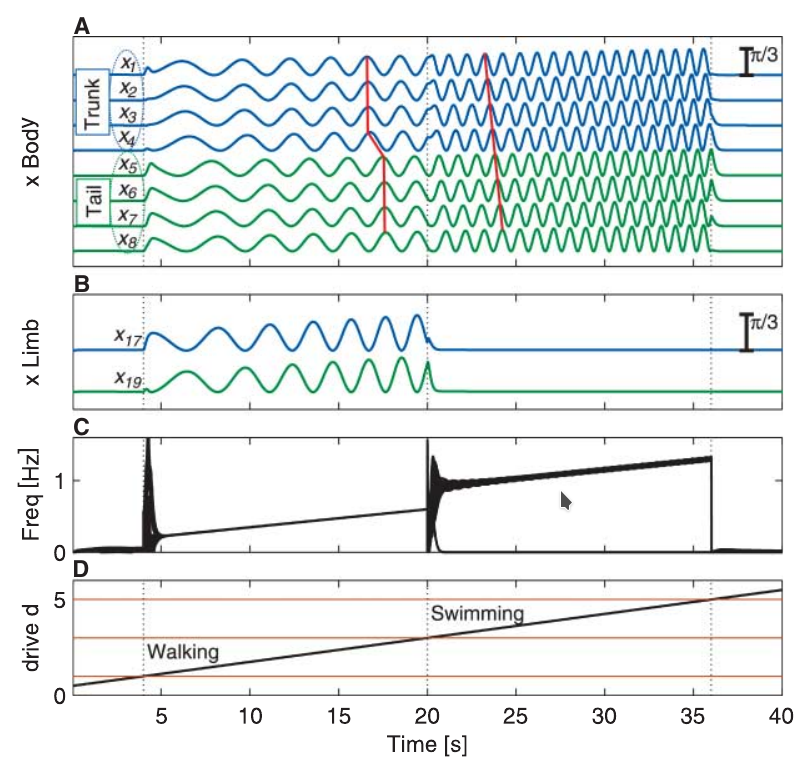
\includegraphics[width=0.7\textwidth]{figures/science_oscillator_patterns}
  \caption{Oscillator patterns from \cite{ijspeert2007swimming}, see
    \cite{ijspeert2007swimming} for details}
  \label{fig:science_oscillator_patterns}
\end{figure}

\begin{figure}[H]
  \centering
  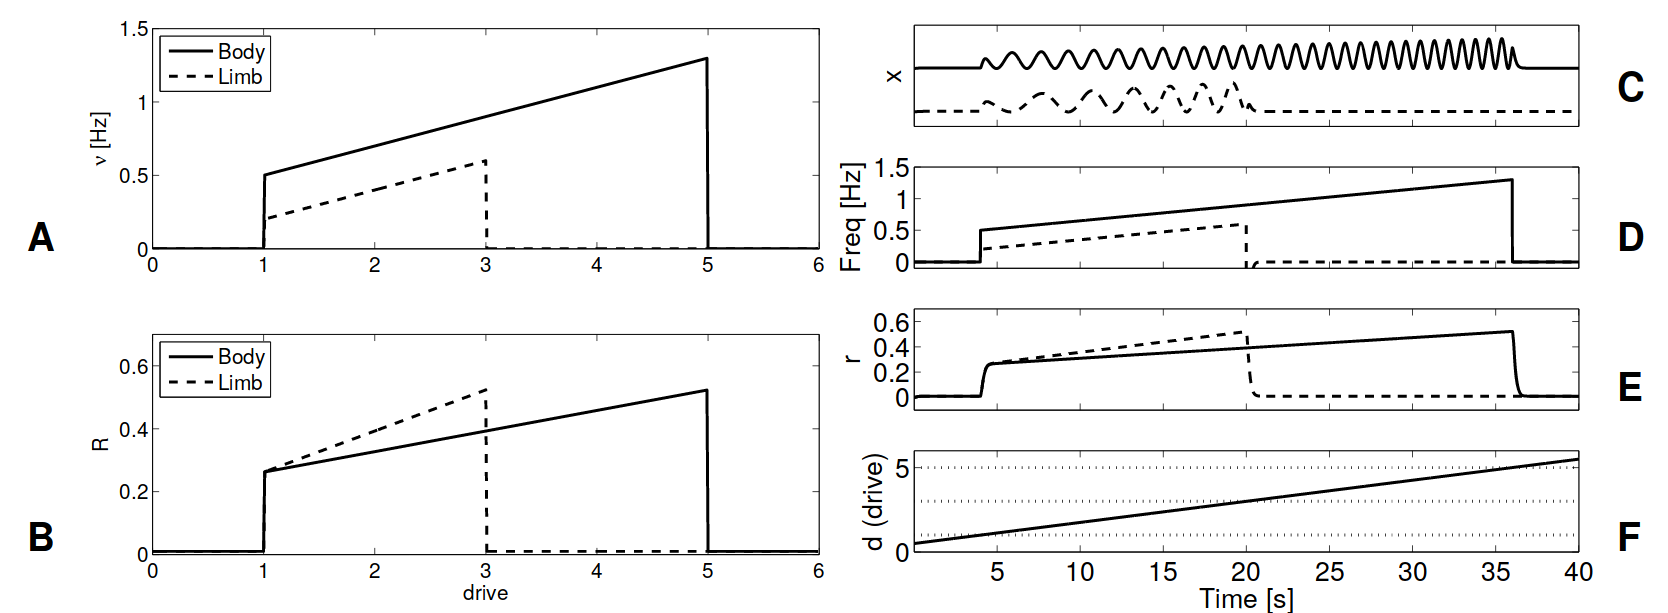
\includegraphics[width=1.0\textwidth]{figures/science_oscillator_properties}
  \caption{Oscillator properties from \cite{ijspeert2007swimming} supplementary
    material, see \cite{ijspeert2007swimming} for details}
  \label{fig:science_oscillator_properties}
\end{figure}


\bibliography{project1}
\label{sec:references}
\bibliographystyle{ieeetr}


% \newpage

% \section*{APPENDIX}
% \label{sec:appendix}

\end{document}

%%% Local Variables:
%%% mode: latex
%%% TeX-master: t
%%% End: